\section{Semantic Web Topics}
The following topics come from the research area of Semantic Web.
Since this thesis focuses mostly on the implementation and deployment of the Basilisk platform, these topics are mostly introduced to give a basic understanding of the context in which the Basilisk platform is used.

\subsection{Knowledge Graphs} 
\label{sec:knowledge_graphs}
Knowledge Graphs are graphs intended to represent knowledge of the real world or smaller scenarios.
The knowledge stored in Knowledge Graphs is modeled in a graph-based structure. 
Nodes represent entities which are connected by various types of relations, represented by labeled edges in the graph.
This has the benefit to represent complex relations between different nodes and edges\cite{hoganKnowledgeGraphs2021}.

The simplest knowledge graph consists of three elements.
The subject entity, the object entity and the labeled edge between them describing their relation.
This atomic data entity is called triple.
In figure \ref{fig:example-knowledge-graph} a simple example of a knowledge graph is shown.

\begin{figure}[tbph]
	\centering
	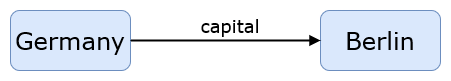
\includegraphics[width=0.4\textwidth]{figures/knowledge-graph-diagram}
	\caption{Simple Knowledge Graph}
	\label{fig:example-knowledge-graph}
\end{figure}

Since a graph structure is hard to store in a classic relational database a different type of storage is needed.
The special kind of database developed to store knowledge graphs are called \tsp{}.


\subsection{RDF}
\label{sec:rdf}
The Resource Description Framework is a framework for describing data and knowledge in a standardized way \cite{RDFConceptsAbstract} and it is part of the W3C standard.
The information is written down as subject-predicate-object triples, representing the basic structure that is also present in Knowledge Graphs (\ref{sec:knowledge_graphs}).
The elements of those triples can be IRIs (internationalized resource identifiers), blank nodes or datatyped literals.

RDF graphs can be encoded with different syntax styles.
A popular syntax is TURTLE \cite{RDFTurtle} which is a compact way of writing down a RDF graph structure.
Using the example of section \ref{sec:knowledge_graphs}, the knowledge graph would be represented with the TURTLE syntax seen in figure \ref{fig:rdf_turtle}.
The first two lines of the TURTLE document define abbreviations for the used IRIs so that the triple in line three is more readable.

\begin{figure}[tbph]
	\begin{lstlisting}
		@prefix dbr: <http://dbpedia.org/resource/> .
		@prefix dbo: <http://dbpedia.org/ontology/> .
		dbr:Germany dbo:capital dbr:Berlin .
	\end{lstlisting}
	\caption{Example of an RDF graph in TURTLE syntax.}
	\label{fig:rdf_turtle}
\end{figure}


\subsection{\ts{}}
\label{sec:triplestores}
\tsp{} are a special kind of database developed to easily store and access knowledge graphs through queries.
Example of \tsp{} are Tentris\cite{bigerlTentrisTensorBasedTriple2020}, GraphDB\footnote{\url{https://graphdb.ontotext.com/}}, Virtuoso\footnote{\url{https://virtuoso.openlinksw.com/}}, or Jena TDB\footnote{\url{https://jena.apache.org/documentation/tdb/}}.

This thesis focuses on \tsp{} that accept SPARQL queries, since the used benchmark framework \iguana{} is using the SPARQL endpoint to perform benchmarks (see section \ref{sec:iguana}).


\subsection{SPARQL}
\label{sec:sparql}
SPARQL (SPARQL Protocol and RDF Query Language)\cite{harrisSPARQLQueryLanguage} is a query language for manipulating and retrieving RDF data stored in \tsp{}.
Just like RDF, SPARQL is part of the W3C recommendations for technologies in the semantic web.

The syntax for SPARQL queries looks similar to the SQL syntax, since its main parts are also a \texttt{SELECT} clause stating which variables to query for, following by an \texttt{WHERE} clause giving restrictions.

Queries can contain optional graph patterns, conjunctions, disjunctions, as well as aggregation functions.
These extension can help formulate more complex queries.

Following the example from section \ref{sec:knowledge_graphs} and \ref{sec:rdf} there are two example SPARQL queries in figure \ref{fig:sparql_example}.
Executed against the DBPedia SPARQL endpoint\footnote{\url{https://dbpedia.org/sparql}} the following results can be found:

The first example query requests the variable which matches the \texttt{WHERE} clause searching for the capital of Germany, which is \texttt{dbr:Berlin}.
The second query requests all relationships that can be found between Germany and Berlin, which will return \texttt{dbo:capital}, which we expected, but also \texttt{dbo:wikiPageLink}, which means that there is a link from the Wikipage of Germany to the Wikipage of Berlin.

\begin{figure}[tbph]
	\begin{lstlisting}
		PREFIX dbr: <http://dbpedia.org/resource/>
		PREFIX dbo: <http://dbpedia.org/ontology/>
		
		SELECT ?capital
		WHERE {
			dbr:Germany dbo:capital ?capital .
		}
		
		---
		
		SELECT ?relation
		WHERE {
			dbr:Germany ?relation dbr:Berlin .
		}
	\end{lstlisting}
	\caption{SPARQL query examples}
	\label{fig:sparql_example}
\end{figure}